%section Y
% Obstacles found

Several obstacles have being delaying the deployment of IPv6 and identifying them has been an important task of the Working Group.
These are the main obstacles that we have been addressing:
\begin{itemize}
  \item Applications don't support or understand IPv6
  \item WLCG Sites not yet deployed IPv6 networking
  \item Sites have IPv6 but Tier-2 has no dual-stack storage
  \item IPv6 monitoring not available or broken
  \item Service is dual-stack but IPv4 being used
\end{itemize}

Support for IPv6 in WLCG application was one of the first obstacles tackled by the Working Group. Applications were first tested on a dual-stack environment and problems were reported to the developers. We maintained a list of the applications with indication of their IPv6 compliance or not. It took a long time, but most of the incompatibility have been removed and today the most important applications work properly with IPv6.

Lack of IPv6 deployment at the sites has been another major obstacle. Deploying IPv6 is relatively easy in a small site, but deploying it at production level in a large site with all the IPv4 functionalities (DNS, firewalling, address management..) is a large and expensive task. Luckily the management of some large site understood the risk of delaying this deployment and made dual-stack networks a reality in several large sites.

But even when sites had IPv6 capable networks, IPv6 traffic was lacking. We soon realized that the most important service to give IPv6 capabilities was storage, so the Working Group proposed to WLCG to mandate the deployment of dual-stack storage. WLCG accepted and we started a GGUS ticket campaign asking every site to report on their progresses.
The campaign is still on-going, but luckily a critical mass was reached quickly and today more than 90% of the LHCOPN traffic is IPv6.

Now that IPv6 was flowing, we soon realized that in many situations it was not possible to measure it. Being storage the main source of network traffic, we have worked with the FTS developers to make it possible to distinguish the IP protocol used for the file transfers. Figure\ref{fig:fts-ipv6} shows a FTS monitoring dashboard in which is visible the moment FTS started distinguishing IPv6 from IPv4.
Other work was done on network monitoring, to distinguish the traffic by protocol on the main network link. In LHCOPN first we used the sflow data generated by the CERN routers, but  once they were replaced to support 400Gbps links, the sflow data became unreliable. So More work was done to separate IPv4 and IPv6 in different VLANs on all the LHCOPN routers.

\begin{figure}[h]
\centering
        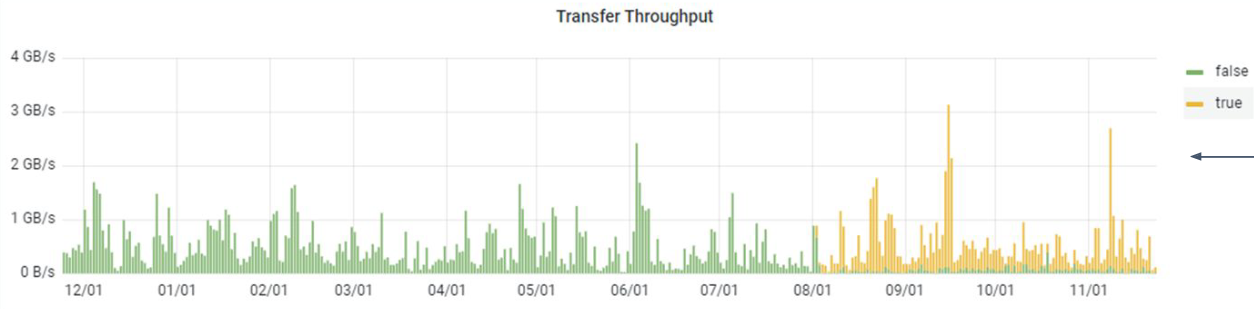
\includegraphics[width=\linewidth]{fts-ipv6.png}
\caption{FTS monitoring now able to distinguish IPv6 from IPv4}
\label{fig:fts-ipv6}
\end{figure}

Another subtle obstacle encountered was that although all the pieces were in place (dual-stack network, software IPv6 capable, service DNS names with correct AAAA records) clients were still preferring IPv4. In most cases it was some hidden or forgotten setting inside the application that forced the use of IPv4.
As an example, figure\ref{fig:aglt2-ipv6} shows  data transfers into USA/ATLAS Great Lakes Tier 2 (AGTL2) where it is possible to see the moment the
variable java.net.preferIPv6Addresses in dCache was set to true.

\begin{figure}[h]
\centering
        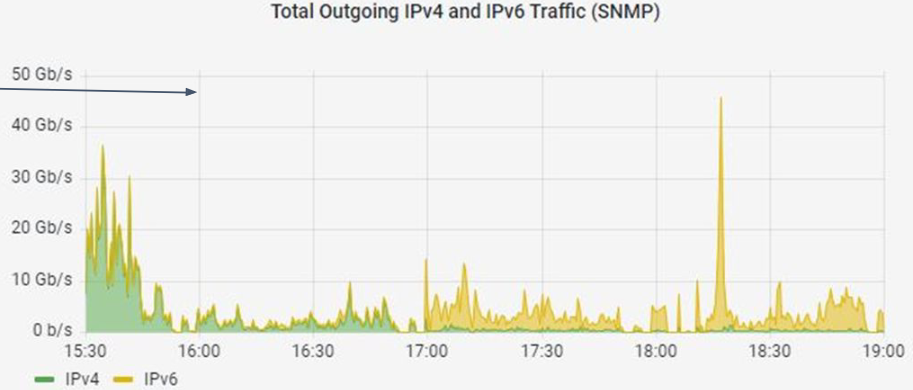
\includegraphics[width=\linewidth]{aglt2-ipv6.png}
\caption{Data transfers into USA/ATLAS Great Lakes Tier 2 (AGTL2)}
\label{fig:aglt2-ipv6}
\end{figure}

%%%% Is the rest part of this section???  %%%%%%%%%%%%%

Obstacles to IPv6 - to be addressed
5. Non-storage services not yet dual-stack
   a. ~60% of all WLCG services are dual-stack today
6. WLCG client CPU (worker nodes, VMs, containers) some IPv4-only
7. Services/clients outside of WLCG Tier-1/Tier-2 not yet considered
   a. Tier-3, Public/Commercial Clouds, Analysis facilities, Experiment portals…
8. Use of new or evolving technologies not yet tested or tracked
   a. New CPU architectures (GPU, non-x86, …), container orchestration, …
9. “People” can be the obstacle
   a. they do not consider use of IPv6 or refuse to deploy!


